\documentclass[conference]{IEEEtran}
\IEEEoverridecommandlockouts
% The preceding line is only needed to identify funding in the first footnote. If that is unneeded, please comment it out.
\usepackage{cite}
\usepackage{amsmath,amssymb,amsfonts}
\usepackage{algorithmic}
\usepackage{graphicx}
\usepackage{textcomp}
\usepackage{xcolor}
\usepackage{float}
\usepackage{subcaption}
\def\BibTeX{{\rm B\kern-.05em{\sc i\kern-.025em b}\kern-.08em
    T\kern-.1667em\lower.7ex\hbox{E}\kern-.125emX}}
\begin{document}

\title{Improved Ant Colony Optimization Algorithm for Robot Path Planning }

    
\author{\IEEEauthorblockN{Syed Muhammad Fasih Hussain}
\IEEEauthorblockA{\textit{Department of Computer Science} \\
\textit{Dhanani School of Science and Engineering} \\
Habib University – Karachi, Pakistan\\
sh05204@st.habib.edu.pk}
\and
\IEEEauthorblockN{Salman Muhammad Younus}
\IEEEauthorblockA{\textit{Department of Computer Science} \\
\textit{Dhanani School of Science and Engineering} \\
Habib University – Karachi, Pakistan\\
sy04351@st.habib.edu.pk}
\and
\IEEEauthorblockN{Muhammad Munawwar Anwar}
\IEEEauthorblockA{\textit{Department of Computer Science} \\
\textit{Dhanani School of Science and Engineering} \\
Habib University – Karachi, Pakistan\\
ma04289@st.habib.edu.pk}
}

\maketitle

\begin{abstract}
Path planning is an active research area for motion control of autonomous robots. Path planning is an NP-complete problem which means that it cannot be solved using traditional algorithms for hard instances. The ACO (Ant Colony Optimization) algorithm is an optimization technique based on swarm intelligence. This report investigates the application of an improved ACO to robot path planning in dynamic and static environments. The simulation in Python shows that improved ACO has higher efficiency for path search.
\end{abstract}

\begin{IEEEkeywords}
Dijkstra Algorithm, A* search Algorithm, Ant Colony Optimization, Path Planning 
\end{IEEEkeywords}

\section{Introduction}
In current society, with the development of computer technology and intelligent computing, human beings are moving towards automation. Robots are extensively used in different fields such as planetary exploration, deep ocean exploration, military, home, and so on. Robots use multiple sensors to perceive the machine parameters and the current environment, to avoid obstacles to reach the destination. \cite{9148277} \\
Path planning is an important issue for the navigation and motion control of autonomous robot manipulators. In computational complexity theory, path planning is classified as an NP-complete problem. That is, the computational time that is required to solve such a problem increases at an exponential rate when the size (or dimension) of the problem increases.\\
Let robot $A$ be a single rigid object moving in a 2D or 3D Euclidean space denoted by $W$, and let obstacles $B$ be rigid objects distributed in W.  Then a path planning problem can be formulated as the following :\\ 
Given an initial position and a goal position  of A in W, generate a path that specifies a sequence of positions of A avoiding contact with B, starting from the initial position and terminating at the goal position. Report failure if no such path exists. \cite{5541300}\\
The studies of path planning started in the late '60s and many different algorithms have been proposed since. Dijkstra, A* search , ACO, etc. are commonly used for path planning algorithms. Dijkstra is a greedy algorithm, which only considers the distance from the current node to the next node, and uses the method, traversal search, to find the shortest path. The obtained path has high reliability and good robustness, but the complexity is high and it is easy to fall into local optimum. Based on Dijkstra, the A* search introduces a heuristic function to guide path searching. However, the traditional A* search gradually determines the next path by comparing the neighborhood heuristic function. When the heuristic function value has multiple minimum values, the A* search algorithm cannot guarantee the best solution for path searching.  Ant colony optimization is an optimization technique based on swarm intelligence. It is a robust technique. However, it has a long searching time and easy to fall into the local optimum.Due to the shortfalls of AC0, this report presents a modified ACO algorithm.  The modified ACO uses the self-adaptive adjustment method to improve the bearing coefficient $\rho$ of pheromone and then updates the improved bearing coefficient into the pheromone update formula of the ACO.\cite{8991502}\\
The rest of this paper is organized as follows. Section II introduces Robot Path Planning. Section III reviews the Ant colony optimization algorithm and the improvement .Section IV describes the proposed algorithm and gives the details of its components. Experimental results and relevant analysis are demonstrated in Section V.  Finally,
conclusions are summarized in Section VI.
\section{Background}
\subsection{Robot Path Planning Problem}
Path planning of autonomous robots can be categorized into four different categories based on the different combinations of environment and obstacles. The environment may be known or unknown. The obstacles can be considered static or dynamic. A dynamic environment is where an optimal path needs to be re-routed when a new obstacle appears. The ultimate goal of path planning is to reduce the distance, cost, or time. In this report, path planning is done for a known environment with static and obstacles using a modified ACO to find best the possible route from the source to the destination avoiding obstacles. \cite{7823281}
\subsection{Grid World}
This article uses the two-dimensional grid method to represent the robot environment, and the grid squares are divided into two types: free grid square, which is represented by zero, and obstacle grid square, which is represented by one. The robot can only move in the free grid. \cite{1621617} The source is denoted by S and the destination is represented by D. The goal of the robot is to move from S to D avoiding the obstacles. Report failure if no such path exists
\begin{figure}[h!]
\centering
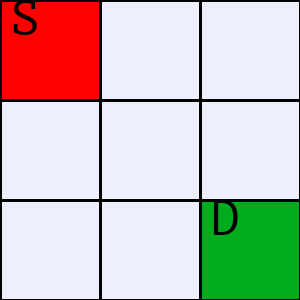
\includegraphics[width=0.3\textwidth]{EviormentGrid.png}
\caption{Representing environment as grid}
\label{fig}
\end{figure}
\newline
The movement of robot is restricted to eight directions is depicted in Figure 2 - North West, North, North East, West, East, South West, South East and South West. 
\begin{figure}[h!]
\centering
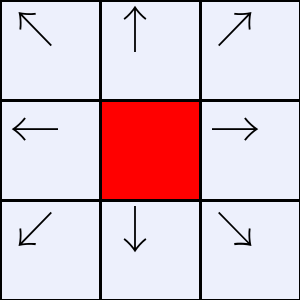
\includegraphics[width=0.3\textwidth]{AgentDirections.png}
\caption{Possible movements of a robot in a free grid}
\label{fig2}
\end{figure}
\section{The Ant Colony Optimization Algorithm}
\subsection{The Basic Idea of Ant Colony Algorithm}
The Ant Colony Optimization ACO was developed by M. Dorigo in 1992 to mimic the behavior of real ants searching for food. When searching for food, ants exhibit complex social behavior by depositing hormones called pheromones.  Pheromones attract other ants and outline a path to the food source that can be followed by other ants. As more ants walk along the path, more pheromone is laid, and the likelihood that other ants will also take the path increases.  The shortest path to the food source will have the highest concentration of pheromone because more ants can travel in the least amount of time. To prevent the convergence to a sub-optimal path, the pheromone also evaporates over time, thereby reducing the chances that other ants to take the path. On the other hand, the pheromone levels on the shortest path remain high, because in this case, the rate at which ants deposit pheromone is greater than the rate of evaporation. \cite{5541300}
\subsection{Mathematical Model}
Consider a given network where ants can travel between different nodes.The probability that  ant $k$ located at node $i$ will choose to go to another node $j$ in the network is given by
\begin{equation}
    p_{ij}^{k} = 
    \begin{cases}
    \frac{(\tau_{ij}^{t})^\alpha (\eta_{ij}^{t})^\beta}{\sum_{l \in N_{i}^{k} } (\tau_{il}^{t})^\alpha (\eta_{il}^{t})^\beta} & \text{ if  } j \in N_{i}^{k}\\
    0 & otherwise
    \end{cases}
\end{equation}
where $\tau_{ij}^{t}$ is pheromone concentration at edge $(i,j)$, $N_{i}^{k}$ the possible set of choices ant $k$ has when at node $i$, and $t$ represents the time step. The values of $\alpha,\beta$, and $\eta_{ij}^{k}$ are usually application dependent; $\eta_{ij}^{k}$ represents the heuristic information and the value of $\alpha$ and $\beta$ weight the importance of the pheromone and heuristic values. 
When $\beta = 0$ , $(\eta_{ij}^{t})^\beta = 1$, then the probability only depends on pheromone levels; on the other hand, when $\alpha=0$, then the probability depends on the heuristic information.

The pheromone levels of the path from node $i$ to node $j$ can evaporate with a percentage $\rho$ (also the called the evaporation rate) where $0 \leq \rho \leq 1$.
\begin{equation}
    \tau_{ij}^{t} = (1 - \rho) \tau_{ij}^{t}
\end{equation}

After the pheromone evaporation occurs, the new pheromone levels are updated with the additional pheromone laid by the ant(s) that just crossed the path:
\begin{equation}
    \tau_{ij}^{t} = \tau_{ij}^{t} + \sum_{k=1}^{m}\Delta \tau_{ij}^{k}
\end{equation}
\begin{equation}
    \Delta \tau_{ij}^{k} = \frac{1}{C^{k}}
\end{equation}
where $C^{k}$ is the associated cost of ant $k$ for choosing this path.
\subsection{Overall structure of the Ant Colony Algorithm}
\begin{figure}[H]
    \centering
    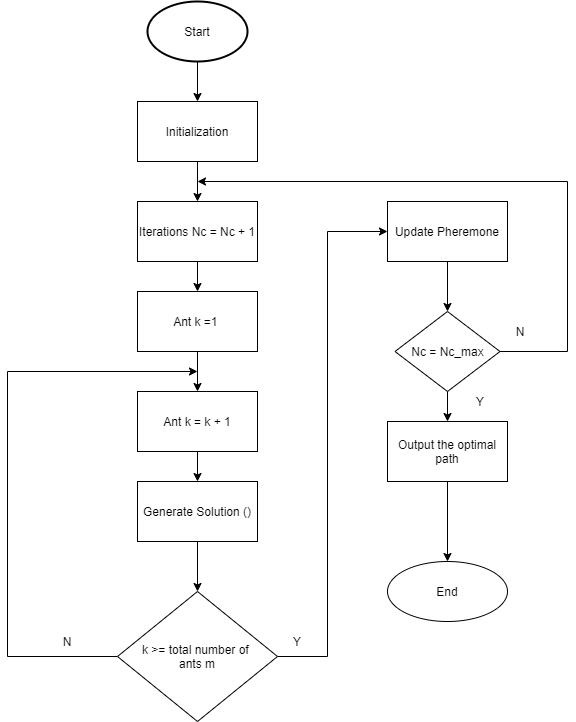
\includegraphics[width=0.35\textwidth]{ACO.png}
    \caption{Computation Flowchart of the ACO}
    \label{fig3}
\end{figure}
\subsection{Improved Ant Colony Algorithm}
Due to the disadvantages that the path searching time of ant colony algorithm is long and it is easy to fall into the local optimal solution, this report presents a self-adaptive adjustment method to improve the bearing coefficient $\rho$ of pheromone, and then updates the improved bearing coefficient into the pheromone update formula of ant colony algorithm \cite{9148277}. 
The formula for improved $\rho$ is as follows: 
\begin{equation}
    \rho_{ij} = e^\frac{\tau_{ij}^{t} min}{\tau_{ij}} + e^{-1}
\end{equation}
where $\tau_{ij}^{t} \mbox{ min }$ refers to the minimum value of pheromone concentration on the edge$(i,j)$ at time t. The overall structure of the algorithm can be seen in Figure \ref{fig4}.
\begin{figure}[H]
    \centering
    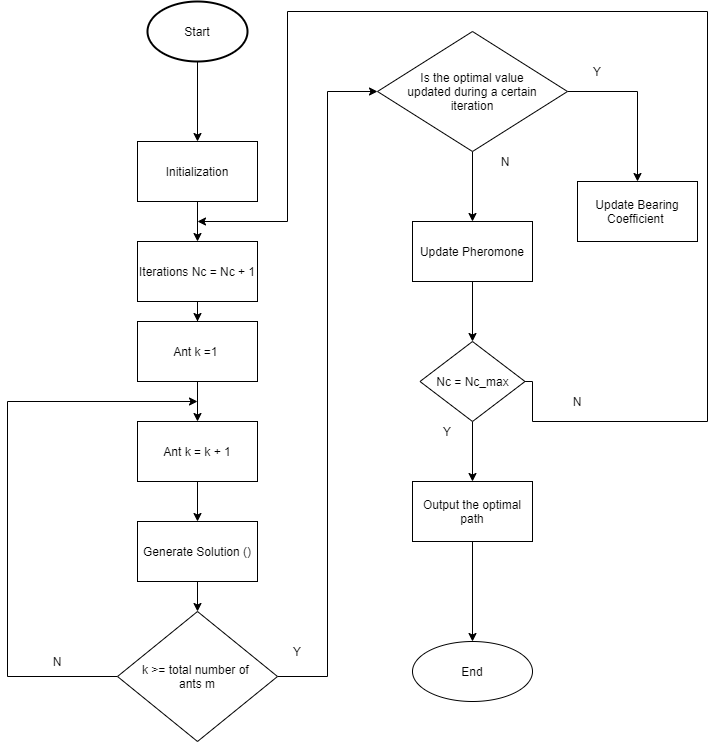
\includegraphics[width=0.35\textwidth]{ImprovedACO.png}
    \caption{Computational Flowchart of Improved ACO}
    \label{fig4}
\end{figure}
\section{Robot Path Planning based on Ant Colony Algorithm}
In this section, the improved ant colony optimization algorithm is applied for robot path planning in a grid network.It is assumed that the one ant can only one node and moves to one of its adjacent nodes at a time in eight different directions. All the nodes are evenly distributed in the network; and distance between any two adjacent nodes is normalized to 1. Thus, path length is represented in terms of the number of unit blocks.The envoirment is known but it can have dynamic or static obstacles. 

The simulation starts with a grid which is populated with obstacles randomly. The number of obstacles added is proportional to the size of the network. All the pheromones are initialized as 0.1 The improved ant colony algorithm is then applied to find the shortest path and pheromones are deposited. 

To simulate a dynamic envoirment, new barriers are added after the algorithm converges. The improved ACO must be called again in order to find the shortest path in this new network with obstacles. The flowchart is show in Figure \ref{fig5}.
\begin{figure}[H]
    \centering
    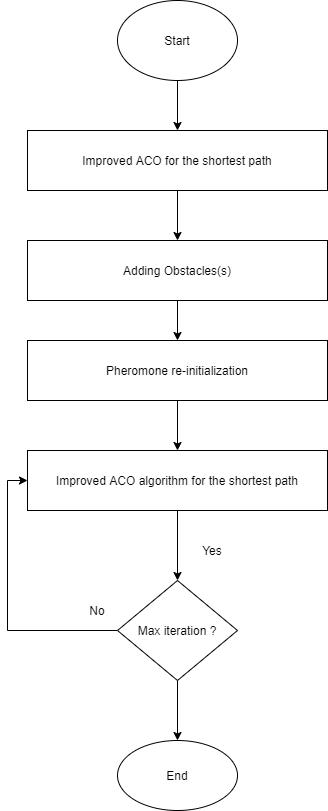
\includegraphics[width=0.2\textwidth]{RobotPathPlanning.png}
    \caption{The flowchart of Improved ACO in a dynamic envoirment}
    \label{fig5}
\end{figure}
\section{Experimental Results of Robot Path Planning}
\subsection{Experimental Setup}
We simulated the four algorithms A*star search, Dijkstra, ACO and Improved ACO in Python with a $4.30 GHz$ processor and $16GB$ Ram. We used the grid sizes of $30 \times 30$, $20 \times 20$,$10 \times10$. We used both static and dynamic obstacles.
\begin{table}[htbp]
\caption{Parameter for the Ant Colony Algorithm}
\begin{center}
\begin{tabular}{|l|l|}
\hline
Parameters                             & Numerical Value \\ \hline
Number of Iterations , $N_c$                   & 50             \\ \hline
Number of ants , $m$                   & 40              \\ \hline
Alpha,$\alpha$                & 1.2             \\ \hline
Beta, $\beta$                        & 0               \\ \hline
Q                                      & 1               \\ \hline
Attenuation coefficient of Pheromone, $\rho$ & 0.6             \\ \hline
Pheromones under initial   conditions, $\tau_{0}$   & 1.5             \\ \hline
\end{tabular}
\label{tab1}
\end{center}
\end{table}

\subsection{Simulation Results}
Our envoirment can be is a grid of $30 \times 30$. Each cell in the grid represents a node in the graph. In this grid, the top most left corner is our destination which is represented by a red dot whereas our origin is the bottom most right corner which is represented by a blue dot. The free grid where the ants can move is represented by the white cells and the obstacles are represented by the black cells. The grid can be seen in $\ref{fig6}$
\begin{figure}[H]
    \centering
    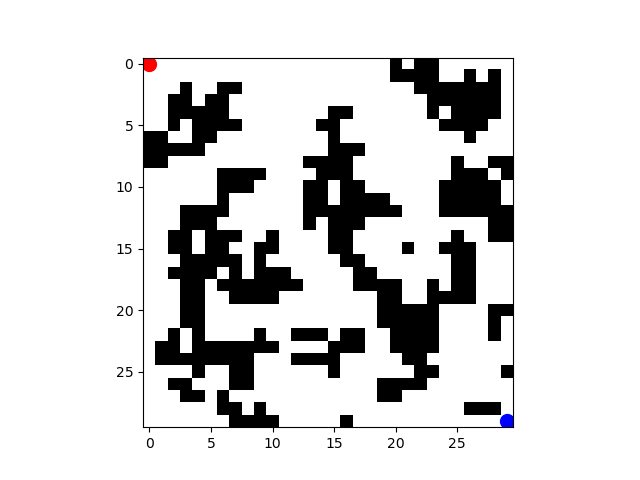
\includegraphics[width=0.4\textwidth]{30x30_grid.png}
    \caption{Static envoirment represented by a $30 \times 30$ grid. }
    \label{fig6}
\end{figure}
After initialising, the shortest path between the source and destination was found using the improved ACO. The path that was returned by the improved by the ACO can be seen in figure \ref{fig7} and is represented by the blue line.
\begin{figure}[H]
    \centering
    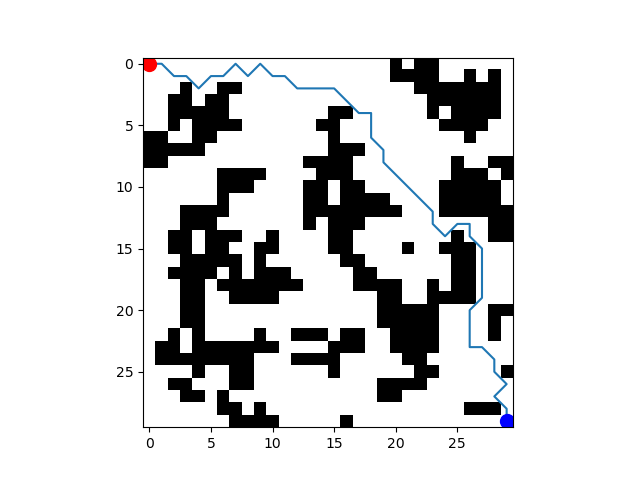
\includegraphics[width=0.4\textwidth]{30x30 grid (ACO Dynamic 1).png}
    \caption{Global shortest path planning results in $30 \times 30$ grid. }
    \label{fig7}
\end{figure}
In order to simulate a dynamic envoirment , the dynamic obstacles are added after the algorithm converges. The new obstacles that were added are represented by red cells and can be seen in figure \ref{fig8}
\begin{figure}[H]
    \centering
    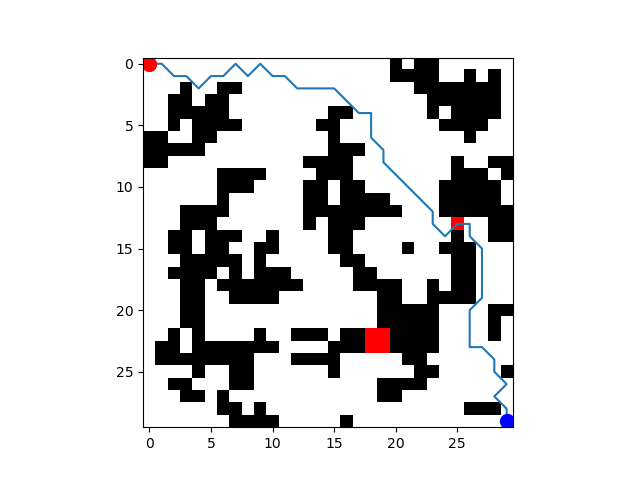
\includegraphics[width=0.4\textwidth]{30x30 grid (ACO Dynamic 2).png}
    \caption{Obstacles avoiding the route of the ants }
    \label{fig8}
\end{figure}
The improved ACO was again called to find the new the shortest path after obstacles were added. The final path of the ants can be seen in figure \ref{fig9}
\begin{figure}[H]
    \centering
    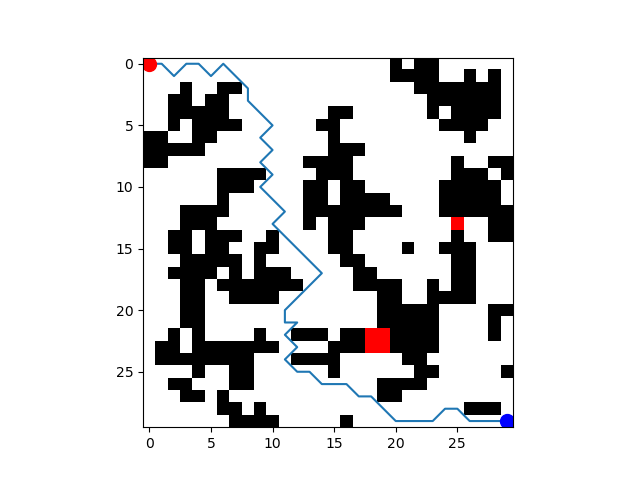
\includegraphics[width=0.4\textwidth]{30x30 grid (ACO Dynamic 3).png}
    \caption{Final Path found by Ants.}
    \label{fig9}
\end{figure}
\subsection{Comparison with other path planning algorithms}
The results that were obtained by running four different algorithms in grid of different sizes with static obstacles are summarised in Table \ref{table2},\ref{table3} and \ref{table4}. The path measured here is measured in number of blocks and the time taken is measured in seconds.

\begin{table}[H]
\caption{STATIC GRID OF 10 BY 10}
\begin{center}
\begin{tabular}{|l|l|l|}
\hline
Algorithm          & Path   Length & Time   Taken(s) \\ \hline
Dijkstra          & 14            & 0.0148          \\ \hline
A*   Search        & 15            & 0.0877          \\ \hline
ACO / Improved ACO & 15            & 0.44            \\ \hline
\end{tabular}
\label{table2}
\end{center}
\end{table}

\begin{table}[H]
\caption{STATIC GRID OF 20 BY 20}
\begin{center}
\begin{tabular}{|l|l|l|}
\hline
Algorithm          & Path   Length & Time   Taken \\ \hline
Dijkstra          & 38            & 0.0974                   \\ \hline
A*   Search        & 38            & 0.0836                   \\ \hline
ACO / Improved ACO & 38            & 2.9                      \\ \hline
\end{tabular}
\label{table3}
\end{center}
\end{table}

\begin{table}[H]
\caption{STATIC GRID OF 30 BY 30}
\begin{center}
\begin{tabular}{|l|l|l|}
\hline
Algorithm            & Path   Length & Time   Taken \\ \hline
Dijkstra            & 43            & 0.4936       \\ \hline
A*   Search          & 44            & 0.0463       \\ \hline
ACO   / Improved ACO & 45            & 4.2          \\ \hline
\end{tabular}
\label{table4}
\end{center}
\end{table}

In figure \ref{fig10}, we can see the shortest paths obtained by Dijkstra, A* search and ACO in the $30 \times 30$ grid with static obstacles. 



\begin{figure}[H]
    \centering
     \begin{subfigure}[b]{0.4\textwidth}
     \centering
         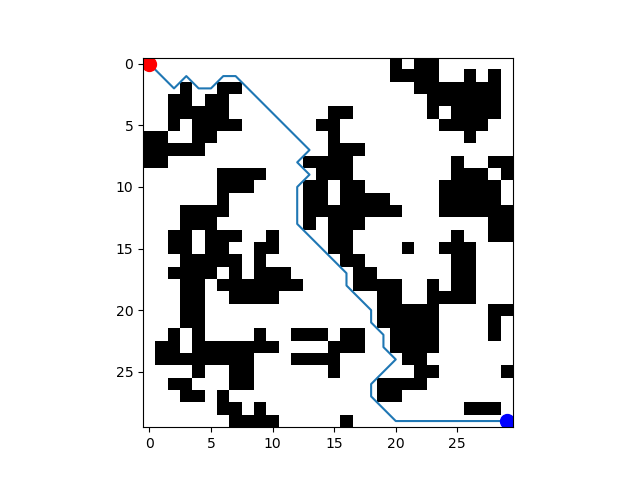
\includegraphics[width=\textwidth]{30x30 grid (A star).png}
         \caption{A* Search}
         \label{fig:x}
     \end{subfigure}
     \hfill
     
     \begin{subfigure}[b]{0.4\textwidth}
     \centering
         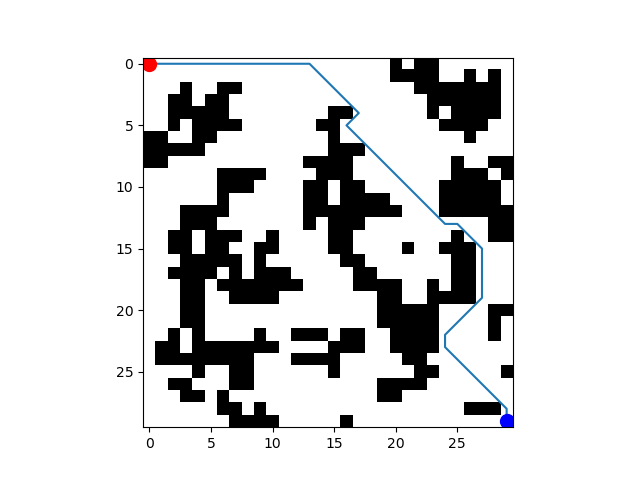
\includegraphics[width=\textwidth]{30x30 grid (dijakstra).png}
         \caption{Dijkstra}
         \label{fig:y}
     \end{subfigure}
     
     \begin{subfigure}[b]{0.4\textwidth}
     \centering
         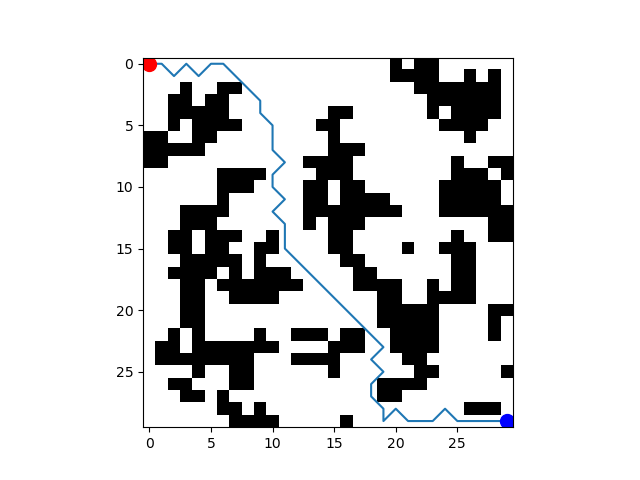
\includegraphics[width=\textwidth]{30x30 grid (ACO improved).png} 
         \caption{ACO}
         \label{fig:xy}
     \end{subfigure}
     
     \caption{Paths obtained in a static grid of size $30 \times 30$}
    \label{fig10}
\end{figure}
The optimal paths found by the traditional ACO were the same as the improved ACO but the improved ACO had a better convergence rate. The results that were obtained are summarised in \ref{table5} and the graphs can be seen in figure \ref{fig11}
\begin{table}[htbp]
\caption{TRADITIONAL ACO VS IMPROVED ACO}
\begin{center}
\begin{tabular}{|l|l|l|l|}
\hline
Size              & 10 BY   10 \ref{fig:110}  & 20 BY   20 & 30 BY   30 \\ \hline
Traditional   ACO & 15         & 20         & 31         \\ \hline
ACO               & 30         & 36         & 42         \\ \hline
\end{tabular}
\label{table5}
\end{center}
\end{table}

\begin{figure}[H]
    \centering
     \begin{subfigure}[b]{0.4\textwidth}
     \centering
         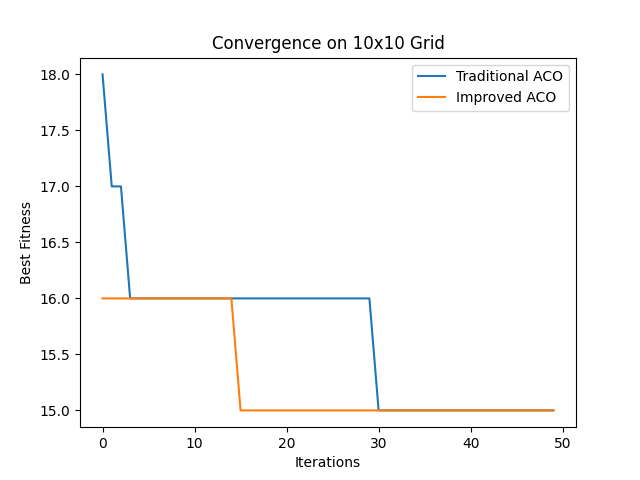
\includegraphics[width=\textwidth]{ACO_Convergence_10x10.png}
         \caption{Static grid of 10 by 10 with static obstacles}
         \label{fig:110}
     \end{subfigure}
     \hfill
     
     \begin{subfigure}[b]{0.4\textwidth}
     \centering
         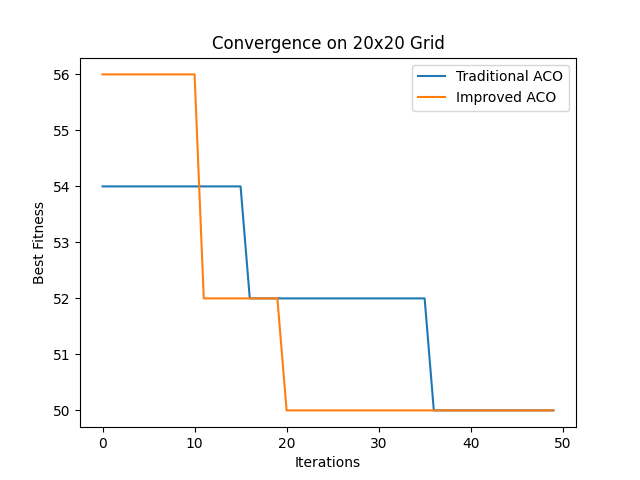
\includegraphics[width=\textwidth]{ACO_Convergence_20x20.png}
         \caption{Static grid of 20 by 20 with static obstacles}
         \label{fig:111}
     \end{subfigure}
     
     \begin{subfigure}[b]{0.4\textwidth}
     \centering
         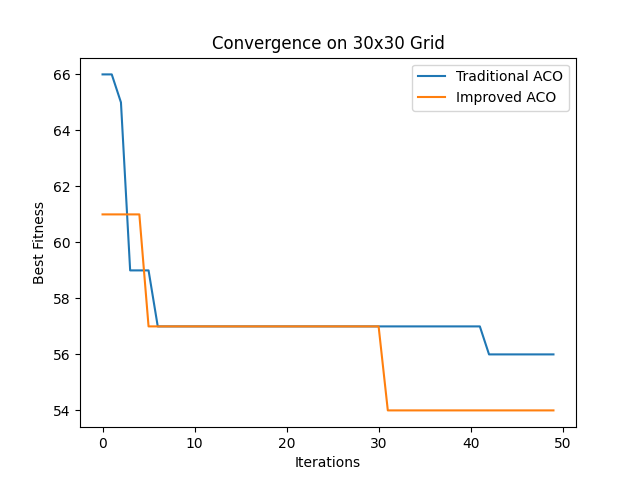
\includegraphics[width=\textwidth]{ACO_Convergence_30x30.png} 
         \caption{Static grid of 30 by 30 with static obstacles}
         \label{fig:112}
     \end{subfigure}
     
     \caption{Convergence rate of ACO vs dynamic ACO}
    \label{fig11}
\end{figure}


\section{Conclusion}

In this paper, we applied four algorithms: Dijkstra,A* Search, ACO and improved ACO to Robot Path planning in a grid world. The improved ACO has the following characteristics: (1) it does not get trapped in a local optima (2) and has a high search efficiency. The performance of this algorithm can be further improved by improving heuristic function and the selection of the next node.
In the future, we would like to focus on multi-robot path 
planning problem in a dynamic envoirment.

\bibliography{references}
\bibliographystyle{plain}


\end{document}
